\chapterimage{header.jpg}
\bigskip
\chapter{Building the WaveWatch III}

 \textbf{This section was written by Dr. Jonas Takeo Carvalho.  \newline Lattes CV: \textit{\textcolor{bleu_cite}{\href{http://lattes.cnpq.br/8827254187143196}{http://lattes.cnpq.br/8827254187143196}}}} 
\bigskip

\section{Generating grids}
\bigskip

 WW3 can be built in many grid options: tradicional regular, curvilinear, triangular unstructured, and spherical multiple-cell (SMC). 
There are some tools been developed and avaiable to built WW3 grids. The example shown here will be focused on tradicional regular grid. Inside 
WW3 \textit{GitHub} page, there is an automated grid generation package for WW3 in \textit{MATLAB} called \textit{gridgen}, avaiable for download along with
the necessary information to use it. The main program \textbf{create\_grid.m} is shown in the figure \textcolor{bleu_cite}{\ref{fig1}}. It is possible to change the grid resolution, 
the latitude and longitude limits, the name of the file generated. Remember to modify the source directories before running. 
\bigskip

 The files generated for this example are:
\bigskip

\begin{itemize}
    \item antartic10km.maskorig\_ascii
    \item antartic10km.depth\_ascii
    \item antartic10km.obstr\_lev1
    \item antartic10km.meta
\end{itemize}
\bigskip

 Respectively the mask file, the bathymetry file, the obstacle file and a grid information file. These files are necessary to compile the WW3 grid 
using the \textbf{{ww3\_grid.inp}} file the executable \textbf{ww3\_grid}, described in the WW3 manual. The resultant file is \textbf{mod\_def.ww3}, that will 
be used for running the model. In figure \textcolor{bleu_cite}{\ref{fig2}}, it is shown the bathymetry generated in this example.
\bigskip

 In future tutorials we intend to show other examples of grid generation, but for now, the most common use within COAWST framework is the tradicional regular 
grid. We also intend to ilustrate how to generate boundary conditions for regional simulations, and how to set a coupled configuration using WW3.  
\bigskip

%Figura1
\begin{figure} [!htb] 
\centering
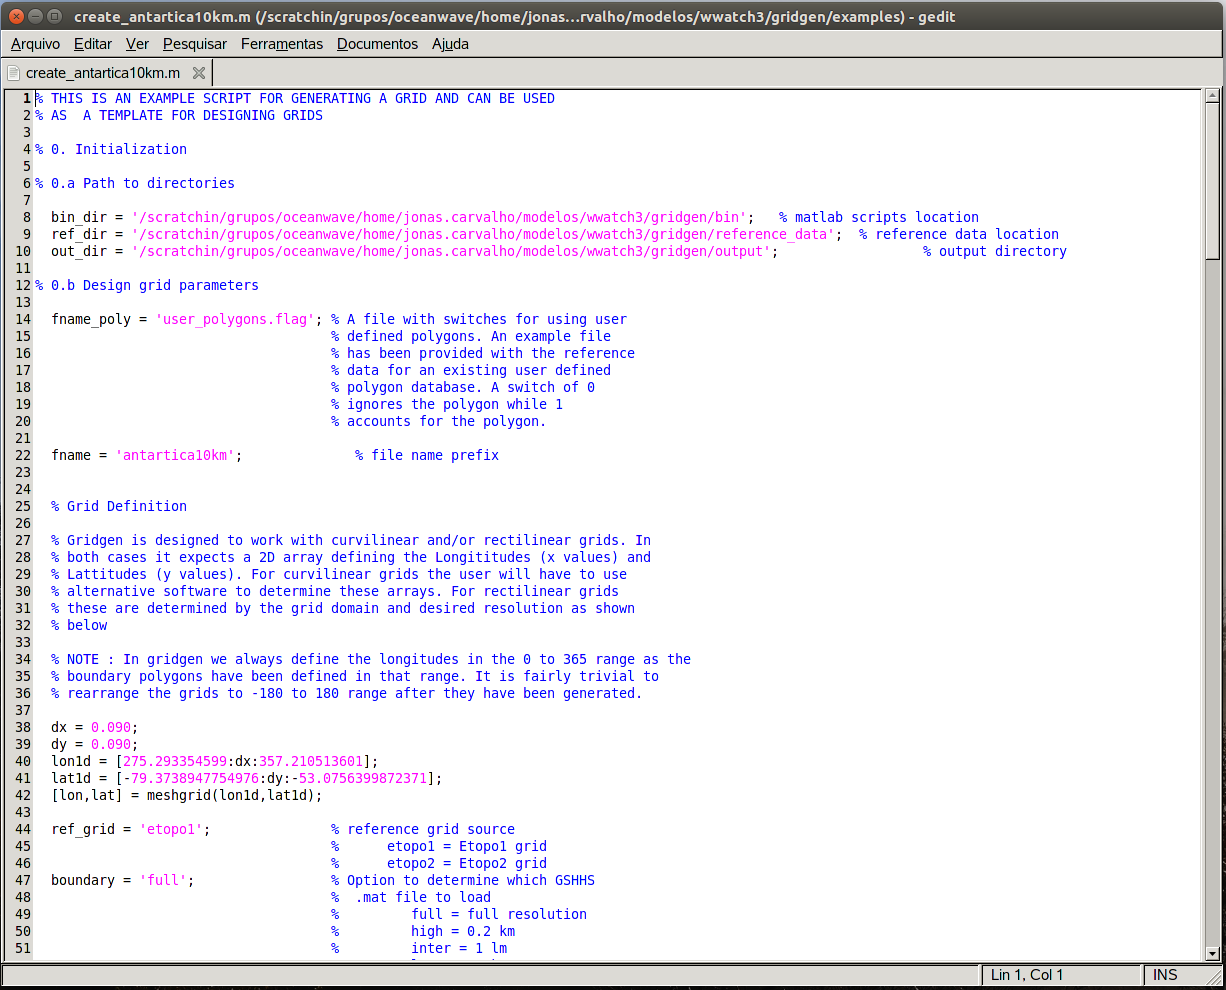
\includegraphics[trim=0.15cm 0.15cm 0.15cm 0.5cm,clip,width=0.75\textwidth]{ww3_ant_grid.png}
\caption{Gridgen main script}
\label{fig1}
\end{figure}


%Figura2
\begin{figure} [!htb] 
\centering
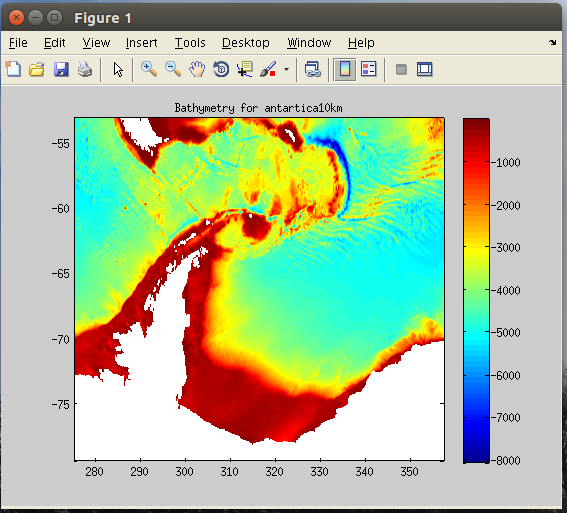
\includegraphics[trim=0.15cm 0.15cm 0.15cm 0.5cm,clip,width=0.75\textwidth]{ww3_ant_bat.png}
\caption{Bathymetry file: antartic10km.depth\_ascii}
\label{fig2}
\end{figure}
